\chapter{Waves, Quantized Modes, and Creation Operators}

\section{Waves, Fields, and Complex Exponentials}

Quantum field theory is the basic tool of particle physics. Before giving even an elementary account of a quantum field, it is useful to collect the mathematical facts that connect waves with particles. A wave is already a field configuration: a field varies from point to point in space, and a wave is a configuration in which those values oscillate and propagate. Quantum mechanics supplies the link between such waves and particles.

Quantum mechanics and special relativity are assumed background here. The immediate purpose is to review the pieces needed for particle physics, not to replace a course in either subject.

An exponential is characterized by proportional growth. If
\begin{equation}
f(x)=e^{\alpha x},
\end{equation}
then
\begin{equation}
\frac{df}{dx}=\alpha f.
\end{equation}
Over a small interval, the increase is proportional to the amount already present. A population growing in a Petri dish gives the familiar picture: the more organisms are present, the more are available to reproduce, so the rate of increase is proportional to the population itself. Multiplying \(e^{\alpha x}\) by an overall constant does not change this defining property.

Sine and cosine oscillate instead of growing. They are the same curve shifted by one quarter of a cycle, and differentiation rotates them into one another:
\begin{align}
\frac{d}{dx}\sin(kx)&=k\cos(kx),\\
\frac{d}{dx}\cos(kx)&=-k\sin(kx).
\end{align}
Neither function alone is an exponential, because its derivative is proportional to the other function. The complex combination does have the exponential property. With \(i^2=-1\),
\begin{align}
\frac{d}{dx}\bigl(\cos(kx)+i\sin(kx)\bigr)
&=-k\sin(kx)+ik\cos(kx)\\
&=ik\bigl(\cos(kx)+i\sin(kx)\bigr).
\end{align}
Therefore
\begin{equation}
e^{ikx}=\cos(kx)+i\sin(kx).
\end{equation}
This identity comes up repeatedly because sines and cosines describe wave-like oscillations. When \(x\) is a spatial coordinate, the function oscillates through space. When the argument is time, it oscillates in time.

\section{Frequency, Wavelength, and Photon Momentum}

The ordinary frequency \(f\) is the number of complete cycles per second. A cycle means one full oscillation. Angular frequency measures the same motion in radians per second:
\begin{equation}
\omega=2\pi f.
\end{equation}
The two notations describe the same frequency. One moves between them to keep unnecessary factors of \(2\pi\) out of a calculation, although the factors never disappear altogether.

The wavelength \(\lambda\) is the distance occupied by one complete spatial cycle. If a wave propagates with speed \(v\), then the distance per cycle times the number of cycles per second is the propagation speed:
\begin{equation}
\lambda f=v.
\end{equation}
For light in vacuum, \(v=c\), so
\begin{equation}
\lambda f=c.
\end{equation}
For a sound wave the right-hand side is the speed of sound, and for a water wave it is the appropriate water-wave speed. The appearance of \(c\) is therefore a statement about light, not a definition common to every wave.

Quantum mechanics introduces Planck's constant in two notations,
\begin{equation}
\hbar=\frac{h}{2\pi}.
\end{equation}
Changing from \(h\) to \(\hbar\) merely moves factors of \(2\pi\) from one equation to another.

The numerical values of dimensional constants depend on the units used to quote them. Metres, seconds, and kilograms are human-scale conventions, convenient for ordinary lengths and times. Traditional units comparable with the length of an arm were useful for cloth or rope; whatever the precise historical route to the metre, no fundamental principle selects this particular human scale. In SI units,
\begin{equation}
\begin{aligned}
h &\simeq 6.6\times10^{-34}\ \mathrm{J\,s},
&\hbar &\simeq 1.1\times10^{-34}\ \mathrm{J\,s},\\
c &\simeq 3\times10^8\ \mathrm{m\,s^{-1}}.
\end{aligned}
\end{equation}
The point of these figures is their scale in conventional units: Planck's constant is extraordinarily small and the speed of light is extraordinarily large.

One quantum of a mode has energy
\begin{equation}
E_{\text{one quantum}}=\hbar\omega=hf.
\end{equation}
This is the energy of one photon, not the total energy of an arbitrary classical electromagnetic wave. Visible light has a frequency of order \(10^{15}\) cycles per second, so a typical optical photon has energy of order
\begin{equation}
E_\gamma\sim 10^{-19}\ \mathrm{J}.
\end{equation}
Even such a rapid optical oscillation gives a very small energy per quantum because \(h\) is so small. A macroscopic amount of optical energy therefore contains an enormous number of photons.

Energy and momentum deserve special attention because both are conserved. They are useful bookkeeping quantities: the total energy and momentum entering a process must be balanced by the total energy and momentum leaving it. Momentum is a vector and points in the direction of motion. For a particle moving much more slowly than light,
\begin{equation}
\vec p=m\vec v.
\end{equation}

Now consider electromagnetic radiation collimated along one direction, rather than dispersed into many directions. Its momentum points along the beam. The nonrelativistic formula cannot be applied to a photon, because \(m\) means rest mass and a photon has zero rest mass. There is nevertheless a useful dimensional mnemonic. If one \emph{inappropriately} assigns the photon the quantity \(E/c^2\) as though it were a mass and then substitutes \(v=c\), one finds
\begin{equation}
mv\longrightarrow \frac{E}{c^2}c=\frac{E}{c}.
\end{equation}
This maneuver happens to give the right answer and gets the units right, but it is not a legitimate argument that a photon has rest mass \(E/c^2\). The actual relativistic statement for collimated radiation is
\begin{equation}
|\vec p|=\frac{E}{c}.
\end{equation}
The equation gives the magnitude. The direction is the direction in which the radiation travels.

For one photon,
\begin{align}
|\vec p_\gamma|
&=\frac{E_\gamma}{c}
=\frac{hf}{c}.
\end{align}
For light,
\begin{equation}
\lambda f=c,
\qquad
\frac{f}{c}=\frac{1}{\lambda},
\end{equation}
and therefore
\begin{equation}
|\vec p_\gamma|=\frac{hf}{c}=\frac{h}{\lambda}.
\end{equation}

\begin{figure}[t]
\centering

\includegraphics[width=0.56\textwidth]{lecture_02_figure_02.png}
\caption{For light, \(\lambda f=c\) and \(f/c=1/\lambda\), the relations used to obtain \(|\vec p_\gamma|=h/\lambda\).}
\lectureframe{00:21:39}
\end{figure}

The shorter the wavelength, the larger the photon momentum. This is one of the most important quantum facts for particle physics. To study a small object one needs a short-wavelength probe, and the price of that short wavelength is large momentum.

\begin{classroomqa}
\lecturetimestamp{00:22:23}
\audiencequestion{Is \(E=\hbar\omega\) fundamental, or is it derived from a deeper principle?}
\lecturerresponse{It follows from the quantum mechanics of the harmonic oscillator. That result will be used here without repeating its proof; the oscillator language developed below gives the deeper setting for it.}
\end{classroomqa}


\section{Wave Amplitude and Photon Number}

\begin{classroomqa}
\lecturetimestamp{00:23:10}
\audiencequestion{What does the amplitude of a wave mean in photon language?}
\lecturerresponse{Compare two waves with the same wavelength and frequency but different amplitudes, such as \(\sin(kx)\) and \(A\sin(kx)\). Classically, the energy in a fixed region is proportional to the amplitude squared. Quantum mechanically, a mode containing \(n\) photons has energy \(n\hbar\omega\). At fixed frequency, region, and normalization, the amplitude therefore grows in order of magnitude like \(\sqrt n\).}
\end{classroomqa}

The two waves are identical in their pattern of oscillation. One is simply stronger than the other.\footnote{The schematic follows the wave comparison at 00:23:47--00:24:28.}

\begin{figure}[t]
\centering
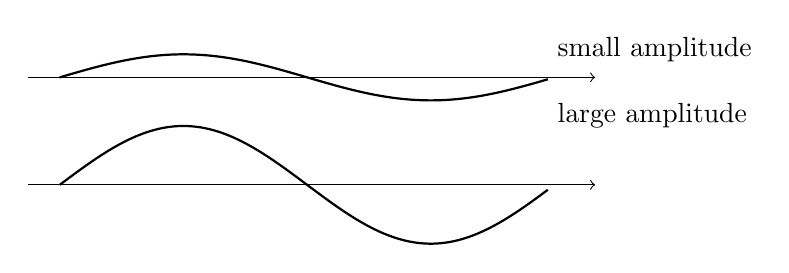
\begin{tikzpicture}[x=1cm,y=0.65cm]
\draw[->] (-0.4,0) -- (6.8,0);
\draw[->] (-0.4,-2.1) -- (6.8,-2.1);
\draw[thick] plot[domain=0:6.2,samples=120] (\x,{0.45*sin(\x r)});
\draw[thick] plot[domain=0:6.2,samples=120] (\x,{-2.1+1.15*sin(\x r)});
\draw (6.2,0.55) node[right]{small amplitude};
\draw (6.2,-0.75) node[right]{large amplitude};
\end{tikzpicture}
\caption{Waves with equal wavelength and frequency but different amplitudes.}
\end{figure}

For a fixed amount of wave,
\begin{equation}
E_{\text{wave}}\propto A^2.
\end{equation}
For an electromagnetic wave this is the familiar statement that field energy is proportional to the square of the field strength. If the same mode contains \(n\) photons, then
\begin{equation}
E_{\text{wave}}=n\hbar\omega.
\end{equation}
Consequently, with the mode, frequency, normalization, and region held fixed,
\begin{equation}
A^2\propto n\hbar\omega,
\qquad
A\propto\sqrt n\quad\text{at fixed }\omega.
\end{equation}
No exact normalization is being asserted. The amount of wave included matters: doubling the length of an otherwise uniform wave changes its total energy without changing the local amplitude. The proportionality may therefore be understood for a fixed region, such as one wavelength.

There is also a specifically quantum qualification. Amplitude and phase cannot both be assigned exact classical values. The question ``What is the amplitude of one photon?'' is therefore ambiguous if it asks for a perfectly sharp classical field. Setting \(n=1\) nevertheless gives a sensible order-of-magnitude scale.

\begin{classroomqa}
\lecturetimestamp{00:28:25}
\audiencequestion{Does the vertical displacement in an electromagnetic-wave drawing represent the photon's position in space?}
\lecturerresponse{No. The propagation axis is spatial, while the vertical coordinate represents the value of the electric or magnetic field. The momentum points along the propagation axis, not along the plotted field amplitude.}
\end{classroomqa}

The wave may propagate in any spatial direction, but the familiar sinusoidal drawing uses only its horizontal axis as a spatial coordinate. The other plotted direction records field strength.

\begin{classroomqa}
\lecturetimestamp{00:29:37}
\audiencequestion{Is the stated photon number being counted within one wavelength or period of the wave?}
\lecturerresponse{One may choose a fixed region such as one wavelength. This is why the relation is only proportional: the total energy and photon number also depend on how much of the wave is included. Two, three, or four wavelengths contain correspondingly more energy than one wavelength at the same amplitude.}
\end{classroomqa}

\begin{classroomqa}
\lecturetimestamp{00:30:17}
\audiencequestion{Is the amplitude of a single photon meaningless?}
\lecturerresponse{It is meaningful only as an order-of-magnitude statement obtained by setting \(n=1\). For an electromagnetic mode, electric- and magnetic-field information plays a role analogous to conjugate position and momentum information, so quantum uncertainty limits how sharply a classical amplitude can be assigned. The order-of-magnitude relation remains useful.}
\end{classroomqa}

These questions already lead into quantum field theory, where the relation between field variables and particle number can be stated precisely. For now the proportionalities are enough.

\section{General Quantum Relations and Slow Matter Waves}

Some formulas introduced for photons apply much more generally, while others do not. It is worth sorting them before turning to electrons.

\begin{figure}[t]
\centering

\includegraphics[width=0.82\textwidth]{lecture_02_figure_03.png}
\caption{Wave definitions and the photon and nonrelativistic momentum relations compared by their domains of validity.}
\lectureframe{00:31:52}
\end{figure}

The definitions of \(f\), \(\omega=2\pi f\), and \(\lambda\) apply generally. The quantum relation
\begin{equation}
E=\hbar\omega=hf
\end{equation}
is also general in the present discussion. By contrast, formulas containing \(c\), such as \(\lambda f=c\) and \(|\vec p|=E/c\), apply to waves moving at the speed of light. The formula \(\vec p=m\vec v\) applies to particles moving much more slowly than light. Relativistic motion between those limits requires an interpolation that is not needed yet.

The momentum--wavelength relation survives the photon example:
\begin{equation}
p=\frac{h}{\lambda}.
\end{equation}
Here \(p\) denotes the magnitude when \(\lambda\) is taken as a positive wavelength; direction can be supplied separately.

\begin{figure}[t]
\centering

\includegraphics[width=0.74\textwidth]{lecture_02_figure_04.png}
\caption{Photon momentum \(|\vec p_\gamma|=hf/c=h/\lambda\), leading to the general de Broglie relation.}
\lectureframe{00:33:32}
\end{figure}

An electron, a nucleus, and even a bowling ball can be associated with a wave. Electron interference is one manifestation of that fact. Write the electron wave as \(\psi\). What replaces \(\lambda f=c\) for a slowly moving electron? The missing ingredient is the nonrelativistic relation between energy and momentum.

Begin with kinetic energy and momentum:
\begin{align}
E&=\frac12 mv^2,\\
p&=mv,
\qquad
v=\frac{p}{m}.
\end{align}
Substituting the last relation into the first gives
\begin{align}
E
&=\frac12m\left(\frac{p}{m}\right)^2\\
&=\frac{p^2}{2m}.
\end{align}
The mass is upstairs in \(\frac12 mv^2\) and downstairs in \(p^2/(2m)\). That placement is easy to confuse and useful to rederive.

Now use the general quantum relations
\begin{equation}
E=hf,
\qquad
p=\frac{h}{\lambda}.
\end{equation}
For a single slow particle,
\begin{align}
hf
&=\frac{p^2}{2m}\\
&=\frac{1}{2m}\left(\frac{h}{\lambda}\right)^2\\
&=\frac{h^2}{2m\lambda^2}.
\end{align}
Dividing by \(h\) yields
\begin{equation}
f=\frac{h}{2m\lambda^2}.
\end{equation}

\begin{figure}[t]
\centering

\includegraphics[width=0.64\textwidth]{lecture_02_figure_05.png}
\caption{For a slow particle, \(E=p^2/(2m)\) and \(p=h/\lambda\) give \(f=h/(2m\lambda^2)\).}
\lectureframe{00:37:47}
\end{figure}

For light,
\begin{equation}
f\propto\frac{1}{\lambda},
\end{equation}
whereas for slow matter,
\begin{equation}
f\propto\frac{1}{\lambda^2}.
\end{equation}
There is no need to memorize the second relation in isolation. It can always be reconstructed from \(E=p^2/(2m)\), \(E=hf\), and \(p=h/\lambda\). For an electron moving slowly in an atom, it gives the frequency of the corresponding Schr\"odinger wave.

\begin{classroomqa}
\lecturetimestamp{00:38:35}
\audiencequestion{Does the nonrelativistic frequency--wavelength relation apply to particles other than electrons?}
\lecturerresponse{Yes. It applies to any particle moving much more slowly than light. The relativistic interpolation between the slow and lightlike limits is a separate subject.}
\end{classroomqa}

\begin{classroomqa}
\lecturetimestamp{00:38:55}
\audiencequestion{Which relation applies to a neutrino?}
\lecturerresponse{It depends on the neutrino's speed. Most neutrinos encountered in nature move very close to the speed of light, so the lightlike relation is a good approximation. A neutrino moving much more slowly than light would instead obey the nonrelativistic relation.}
\end{classroomqa}

\editorialnote{A brief audience exchange immediately after the neutrino question concerns amplitudes, quanta, and differing electron wavelengths, but its wording is too damaged to recover securely. The recoverable response postpones the general relation between amplitudes and quanta of different wavelengths.}

\begin{classroomqa}
\lecturetimestamp{00:39:56}
\audiencequestion{Is an electron from a \(20\,\mathrm{keV}\) accelerator slow or relativistic?}
\lecturerresponse{It is treated as slow. In units with \(c=1\), mass, energy, and momentum can be expressed in the same units. The electron rest-energy scale is roughly \(0.5\,\mathrm{MeV}\), while \(20\,\mathrm{keV}\) is much smaller. Equivalently, the nonrelativistic momentum criterion is \(p\ll mc\).}
\end{classroomqa}

The energy comparison in the example is
\begin{equation}
K=20\,\mathrm{keV}\ll m_ec^2\simeq0.5\,\mathrm{MeV}.
\end{equation}
\editorialnote{The source passage at 00:39:56--00:41:40 introduces \(20\,\mathrm{keV}\) as an accelerator energy and then phrases the relativistic criterion in terms of momentum compared with rest mass. Writing the kinetic-energy and momentum criteria separately avoids identifying the quoted energy with a momentum while preserving the stated nonrelativistic conclusion.}

\section{Phase Velocity, Group Velocity, and Dispersion}

\begin{classroomqa}
\lecturetimestamp{00:41:46}
\audiencequestion{Can frequency times wavelength be used to obtain the velocity of an electron wave?}
\lecturerresponse{It gives the phase velocity, not the velocity assigned to the electron. A localized packet has both a phase velocity, describing the motion of its internal crests and troughs, and a group velocity, describing the motion of the envelope. The group velocity is identified with the particle's motion.}
\end{classroomqa}

A wave packet looks locally like a sine or cosine but is confined by an envelope. As it moves, the envelope and the crests inside it need not move at the same speed.\footnote{The schematic follows the wave-packet discussion at 00:42:34--00:44:11.}

\begin{figure}[t]
\centering
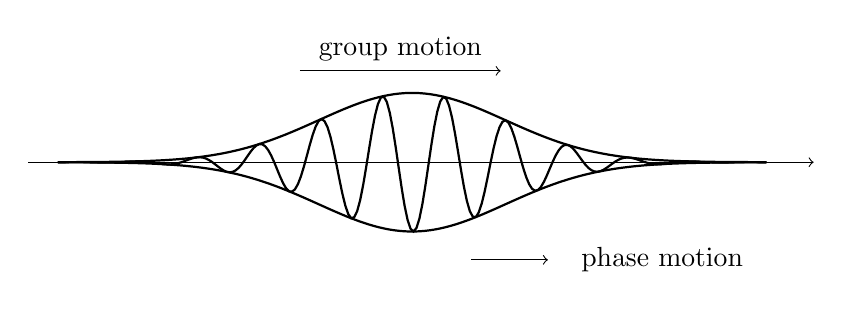
\begin{tikzpicture}[x=0.75cm,y=0.8cm]
\draw[->] (-0.5,0) -- (12.8,0);
\draw[thick] plot[domain=0:12,samples=140] (\x,{1.10*exp(-0.20*(\x-6)^2)});
\draw[thick] plot[domain=0:12,samples=140] (\x,{-1.10*exp(-0.20*(\x-6)^2)});
\draw[thick] plot[domain=0:12,samples=240] (\x,{1.10*exp(-0.20*(\x-6)^2)*sin(6*\x r)});
\draw[->] (4.1,1.45) -- (7.5,1.45);
\draw (5.8,1.8) node{group motion};
\draw[->] (7.0,-1.55) -- (8.3,-1.55);
\draw (8.7,-1.55) node[right]{phase motion};
\end{tikzpicture}
\caption{A localized wave packet whose envelope and internal phase generally move at different velocities.}
\end{figure}

The phase velocity is the velocity of the peaks, troughs, and other fixed phases of a monochromatic component. For the nonrelativistic dispersion relation,
\begin{equation}
v_\phi=f\lambda=\frac{h}{2m\lambda}.
\end{equation}
It depends on wavelength. Different wavelength components therefore have different phase velocities, so the crests can move through the packet and the packet can disperse. The group velocity is the velocity of the packet as a whole, and it is the one identified with the particle.

There is a simple special case. If all wavelength components move with the same velocity, phase and group velocities agree. Light in vacuum has this property: every wavelength propagates at \(c\). The slow-particle relation does not; its \(f\lambda\) changes with \(\lambda\).

The equation
\begin{equation}
f=\frac{h}{2m\lambda^2}
\end{equation}
is the free Schr\"odinger equation in a slightly disguised form. Frequency specifies the temporal dependence of a plane wave, wavelength specifies its spatial dependence, and the Schr\"odinger equation relates the two. Conversely, inserting a definite-frequency, definite-wavelength wave into the free Schr\"odinger equation reproduces this dispersion relation.

\begin{classroomqa}
\lecturetimestamp{00:47:02}
\audiencequestion{Can the phase velocity exceed the speed of light?}
\lecturerresponse{Yes. Phase velocity does not carry information. Information and the localized packet propagate with the group velocity, so a superluminal phase velocity does not permit superluminal signaling.}
\end{classroomqa}

\section{Finite Space and Discrete Momentum}

The eventual interest is in waves in an infinite space, but a finite system is the safer starting point. Infinity is not something a computer can store or manipulate directly. One first formulates the equations for a finite system and only afterward takes the limit in which its size becomes arbitrarily large. This habit is useful throughout quantum mechanics, quantum field theory, and particle physics.

Nothing essential is lost by beginning in one spatial dimension. The wave might live on a violin string, on a rope being shaken, or in an abstract one-dimensional world. The most obvious finite system is a segment of length \(L\) with reflecting ends. A wave travels to an end, reflects, and travels back. This is a perfectly legitimate reflecting boundary condition, but it has an inconvenience: momentum is not conserved within the wave system. A right-moving wave carries rightward momentum; after reflection it carries leftward momentum. The boundary has supplied the impulse and absorbed the difference.

The momentum reversal at a reflecting end can be represented schematically.\footnote{The schematic follows the reflecting-boundary argument at 00:49:24--00:51:08.}

\begin{figure}[t]
\centering
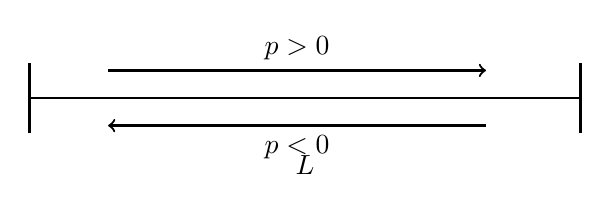
\begin{tikzpicture}[x=1cm,y=1cm]
\draw[thick] (0,0) -- (7,0);
\draw[very thick] (0,-0.45) -- (0,0.45);
\draw[very thick] (7,-0.45) -- (7,0.45);
\draw[->,thick] (1.0,0.35) -- (5.8,0.35) node[midway,above]{\(p>0\)};
\draw[->,thick] (5.8,-0.35) -- (1.0,-0.35) node[midway,below]{\(p<0\)};
\draw (3.5,-0.85) node{\(L\)};
\end{tikzpicture}
\caption{Reflection at the ends of a finite segment reverses the momentum of a traveling wave.}
\end{figure}

There is a different way to make the system finite while preserving momentum. Identify the two endpoints of the segment. It is possible to draw the result as a circle, but no literal circle embedded in a second dimension is required. The mathematical statement is simply that the coordinate is periodic: after traveling a total distance \(L\), one returns to the same point.

\begin{figure}[t]
\centering

\includegraphics[width=0.72\textwidth]{lecture_02_figure_06.png}
\caption{A one-dimensional path of total length \(L\) used to introduce periodic identification.}
\lectureframe{00:51:21}
\end{figure}

The endpoint identification is made explicit in the following schematic.\footnote{The schematic follows the periodic-identification argument at 00:51:09--00:52:37.}

\begin{figure}[t]
\centering
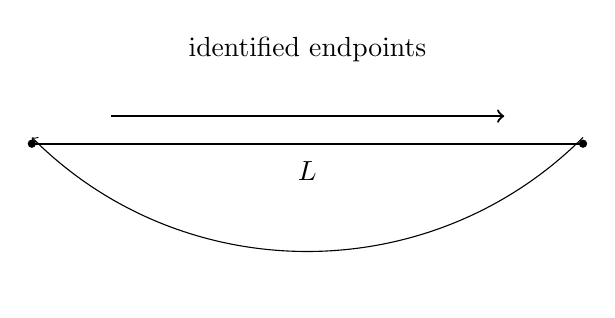
\begin{tikzpicture}[x=1cm,y=1cm]
\draw[thick] (0,0) -- (7,0);
\fill (0,0) circle (1.5pt);
\fill (7,0) circle (1.5pt);
\draw[->,thick] (1.0,0.35) -- (6.0,0.35);
\draw (3.5,-0.35) node{\(L\)};
\draw[->,bend left=45] (7,0.08) to (0,0.08);
\draw (3.5,1.2) node{identified endpoints};
\end{tikzpicture}
\caption{Periodic one-dimensional space formed by identifying the endpoints of a path of length \(L\).}
\end{figure}

A wave moving to the right then reaches the displayed endpoint, reappears at the beginning, and keeps moving to the right. A left-moving wave likewise keeps moving to the left. There is no distinguished endpoint at which the wave reflects, so the momentum does not reverse. Periodic space makes the volume finite and preserves momentum, but it has an important consequence: the allowed momenta are discrete.

An integer number of wavelengths must fit into the total length. For a nonconstant mode,
\begin{equation}
\lambda_{|N|}=\frac{L}{|N|},
\qquad |N|=1,2,3,\ldots .
\end{equation}
Thus the wavelength magnitude can be \(L\), \(L/2\), \(L/3\), and so on. A choice such as \(L/\sqrt{2}\) does not fit: after one circuit the wave would return with the wrong phase and fail to match its starting value.

Using \(p=h/\lambda\), the magnitude of the momentum for the \(|N|\)-th nonconstant mode is
\begin{equation}
|p_N|=\frac{|N|h}{L}.
\end{equation}
To include both directions and the constant mode without ambiguity, it is convenient to let the mode label be signed:
\begin{equation}
p_N=\frac{Nh}{L},
\qquad N=0,\pm1,\pm2,\ldots .
\end{equation}
Positive and negative \(N\) describe opposite propagation directions. The \(N=0\) mode is constant and has zero momentum; it has no finite wavelength to insert into \(h/\lambda\). The basic momentum spacing is therefore \(h/L\).

For a macroscopic \(L\), both \(h\) and \(1/L\) make this spacing extremely small, so the allowed values form a very dense set and look nearly continuous. A bead constrained to a circular wire nevertheless has exactly this discrete spectrum.

\begin{classroomqa}
\lecturetimestamp{00:58:27}
\audiencequestion{Is the quantized quantity the total momentum of the wave, or the momentum associated with one period?}
\lecturerresponse{The statement applies to the momentum of each quantum. Every quantum has one of the allowed discrete momenta. The total momentum of any collection of quanta is consequently also an integer multiple of the basic unit \(h/L\).}
\end{classroomqa}

\begin{classroomqa}
\lecturetimestamp{00:59:22}
\audiencequestion{Why must the wave return to the same value after one circuit?}
\lecturerresponse{The identified endpoints are the same physical point, so an observable field must have the same value there. A mismatch would require a sudden jump in the field at that point. Such a discontinuity is costly in energy and momentum; the admissible field configurations are continuous and periodic.}
\end{classroomqa}

\begin{classroomqa}
\lecturetimestamp{01:00:09}
\audiencequestion{What happens if the wave is localized in a packet?}
\lecturerresponse{A packet is a Fourier sum of plane waves, or equivalently of sines and cosines. In periodic space that sum may contain only the discrete allowed momentum modes. The quantization statement is therefore a statement about the Fourier components of every admissible packet.}
\end{classroomqa}

\begin{classroomqa}
\lecturetimestamp{01:01:01}
\audiencequestion{Is there a problem if the periodic length \(L\) becomes extremely small?}
\lecturerresponse{As \(L\) decreases, the basic momentum \(h/L\) becomes very large. No immediate inconsistency is implied at ordinary microscopic lengths, but attempting to push the construction to the Planck-length regime is expected to require new physics.}
\end{classroomqa}

Now take the circular picture literally: a bead moves on a circular wire of radius \(r\), whose circumference is \(L=2\pi r\). Its allowed tangential momenta are
\begin{equation}
p_N=\frac{Nh}{2\pi r}=\frac{N\hbar}{r}.
\end{equation}
For a nonrelativistic particle in a circular orbit the angular momentum is \(mvr\). Since \(p=mv\) in that regime, this is \(rp\). The expression \(mvr\) is not relativistically general, because \(p\) is then not simply \(mv\), but momentum times perpendicular distance remains the right relation. In vector form,\footnote{The lecture first uses \(L\) for angular momentum, then notices its collision with \(L\) for the periodic length and changes symbols. Here \(J\) is used throughout; see 01:03:40--01:05:21.}
\begin{equation}
\vec J=\vec r\times\vec p,
\end{equation}
and for tangential circular motion its magnitude is \(J=rp\). Hence
\begin{equation}
J_N=rp_N=N\hbar.
\end{equation}
The spacing of linear momentum depends on the size of the circle, whereas the angular-momentum unit is always \(\hbar\). There are exceptions to the integer rule when fermions are involved; those exceptions are postponed.

The next task is to connect fields with particles and quanta more precisely. That requires a short return to the quantum mechanics of operators and the harmonic oscillator.

\section{Wave Modes and Quantum Operators}

The quantum mechanics that follows is necessarily abstract and is meant as a review. The harmonic oscillator is the essential system because a wave is an oscillation. At a fixed point, an electric field, a magnetic field, or any other wave amplitude varies periodically in time; to say that a component has a frequency is already to say that it oscillates.

A general wave need not have only one wavelength. Light of several colors can be mixed together, and, conversely, a prism can separate mixed light into its component colors, as in Newton's decomposition of white light. Each component has its own wavelength, frequency, amplitude, energy, and momentum. Thus the mixed wave may be resolved into quanta of different energies and momenta. Each wavelength determines a frequency, and each definite-frequency component behaves as an oscillator. This is why the harmonic oscillator, rather than an arbitrary quantum system, is the natural building block for a field.

Quantum observables are represented by operators. Operators can be added and multiplied, but unlike ordinary numbers their products need not be independent of order. Let \(A\) and \(B\) represent two properties of a system, each of which might be measurable by itself. For example, \(A\) might represent an electric field and \(B\) a magnetic field. If the measured values are the ordinary numbers \(a\) and \(b\), then
\begin{equation}
ab=ba.
\end{equation}
Their numerical product cannot depend on the order of multiplication. In quantum mechanics, however, the corresponding operators may instead satisfy \(AB-BA\neq0\).

At first this seems nonsensical. If measuring the electric field gives one number and measuring the magnetic field gives another, multiplying those two numbers must give the same result in either order. The resolution is that when the operator products depend on order, the two quantities cannot be measured simultaneously. The experiment that measures one interferes with the measurement of the other. There is no contradiction because the two numerical values cannot be obtained together.

When two quantities can be measured simultaneously, their measured values are ordinary numbers, and those numbers commute. The test for simultaneous measurability is therefore the commutator
\begin{equation}
[A,B]=AB-BA.
\end{equation}
A vanishing commutator means that the observables are compatible; a nonzero commutator means that the corresponding measurements interfere. Reversing the entries reverses the sign:
\begin{equation}
[B,A]=-[A,B].
\end{equation}

For a nonrelativistic particle, the three position components commute with one another, and so do the three momentum components:
\begin{align}
[x,y]&=[y,z]=[z,x]=0,\\
[p_x,p_y]&=[p_y,p_z]=[p_z,p_x]=0.
\end{align}
All three coordinates can be specified together, and all three momentum components can be specified together. Corresponding position and momentum components do not commute:
\begin{equation}
[x,p_x]=[y,p_y]=[z,p_z]=i\hbar,
\end{equation}
whereas mixed components such as \([x,p_y]\) vanish. Measuring a position coordinate gives the particle a disturbance in the conjugate momentum. Equivalently, the product of the corresponding position and momentum uncertainties is controlled by \(\hbar\).

\begin{classroomqa}
\lecturetimestamp{01:16:30}
\audiencequestion{When changing from \(x\) to \(y\), should the \(i\) in the commutator change to \(j\)?}
\lecturerresponse{No. The symbol \(i\) is always the imaginary unit, the square root of minus one. It is neither a Cartesian unit-vector label nor one of the quaternionic symbols \(i,j,k\).}
\end{classroomqa}

\begin{classroomqa}
\lecturetimestamp{01:17:24}
\audiencequestion{Does \(AB-BA\) mean measuring \(A\) first and then \(B\), and then reversing the measurement order?}
\lecturerresponse{No. The two terms are operator or matrix products in different algebraic orders. They do not denote a literal sequence of measurements. The connection with incompatible measurements is a consequence of the operator algebra, not the definition of the product.}
\end{classroomqa}

\begin{classroomqa}
\lecturetimestamp{01:18:32}
\audiencequestion{Do these position--momentum commutators apply directly to a photon?}
\lecturerresponse{Not directly. They apply cleanly to nonrelativistic particles. A photon's position is harder to define, so the analogous statement requires more care and is not needed here.}
\end{classroomqa}

\section{The Quantum Harmonic Oscillator}

A weight on a spring, a sound wave, and a light wave all provide examples of oscillatory motion. Every ideal harmonic oscillator has a frequency. For a spring, one full period is not merely the time required for the weight to return to the same position; it must return to that position moving in the same direction. The number of complete periods per second is \(f\), and \(\omega=2\pi f\).

Classically, an ideal oscillator can have any nonnegative energy. A gentle push gives a small energy, and a harder push gives a larger one. A real spring would eventually break or melt, but the mathematical idealization has a continuous range of positive energies. The quantum oscillator is different: its allowed energies form a discrete, equally spaced ladder. Choosing the origin of energy so that the lowest level is called zero,
\begin{equation}
E_n=n\hbar\omega,
\qquad n=0,1,2,\ldots .
\end{equation}
The equally spaced levels can be pictured as follows.\footnote{The energy-level schematic follows the board discussion at 01:21:20--01:23:56.}

\begin{figure}[t]
\centering
\begin{tikzpicture}[x=1cm,y=0.9cm]
\draw[->] (0,0) -- (0,5.35);
\draw (0,5.5) node[above]{energy};
\foreach \y/\lab in {0.6/{0},1.6/{\hbar\omega},2.6/{2\hbar\omega},3.6/{3\hbar\omega},4.6/{n\hbar\omega}}
{
  \draw[thick] (0.2,\y) -- (2.2,\y);
  \draw (-0.25,\y) node[left]{\(\lab\)};
}
\draw[->,thick] (2.8,0.68) -- (2.8,1.52);
\draw (3.2,1.1) node[right]{\(a_+\)};
\draw[->,thick] (3.7,1.52) -- (3.7,0.68);
\draw (4.1,1.1) node[right]{\(a_-\)};
\end{tikzpicture}
\caption{Equally spaced oscillator levels in the convention \(E_n=n\hbar\omega\).}
\end{figure}

The spacing \(\hbar\omega\) is the same energy assigned earlier to one photon of angular frequency \(\omega\). The value \(2\hbar\omega\) might be the energy of one quantum belonging to an oscillator of frequency \(2\omega\), or the energy of two quanta in an oscillator of frequency \(\omega\). The second interpretation is the one needed here. A single oscillator of fixed frequency may contain zero, one, two, three, or more quanta, with no allowed energies between the rungs.

The integer \(n\) labels the oscillator state, written as a ket \(|n\rangle\). The state \(|0\rangle\) is the ground state, \(|1\rangle\) has one quantum of excitation, \(|2\rangle\) has two, and so on. The ket is simply the notation for the state on which operators act.

Define a raising operator \(a_+\) that moves a state up one level and a lowering operator \(a_-\) that moves it down one level:
\begin{align}
a_+|n\rangle &= \sqrt{n+1}\,|n+1\rangle,\\
a_-|n\rangle &= \sqrt{n}\,|n-1\rangle.
\end{align}
The numerical square-root factors are part of the definitions. On the lowest state,
\begin{equation}
a_-|0\rangle=0,
\end{equation}
because there is no state below the ground state.

It is important here to distinguish ordinary numbers from operators. The label \(n\) and coefficients such as \(\sqrt n\) are ordinary numbers; they commute with everything. The symbols \(a_+\) and \(a_-\) are operators, and their order must be preserved.

First lower \(|n\rangle\), then raise it again. The lowering step gives
\begin{equation}
a_-|n\rangle=\sqrt n\,|n-1\rangle.
\end{equation}
Acting with \(a_+\) on the resulting state supplies another factor \(\sqrt n\), because raising \(|n-1\rangle\) returns it to \(|n\rangle\):
\begin{align}
a_+a_-|n\rangle
&=a_+\bigl(\sqrt n\,|n-1\rangle\bigr)\\
&=\sqrt n\,\sqrt n\,|n\rangle\\
&=n|n\rangle.
\end{align}
Thus \(a_+a_-\) reads the level number. For example, suppose \(|\chi\rangle\) is known to be a number eigenstate but its level label is unknown. If
\begin{equation}
a_+a_-|\chi\rangle=q|\chi\rangle,
\end{equation}
then the ordinary numerical coefficient \(q\) is the number of quanta in that state. The product is therefore the number operator,
\begin{equation}
\hat n=a_+a_-,
\end{equation}
and, in the chosen energy convention, the Hamiltonian is
\begin{equation}
H=\hbar\omega\,a_+a_-.
\end{equation}
Indeed, acting on any level gives \(H|n\rangle=n\hbar\omega|n\rangle\).

Now reverse the order. Raising first gives \(\sqrt{n+1}|n+1\rangle\). Lowering then returns to \(|n\rangle\) and supplies a second factor \(\sqrt{n+1}\):
\begin{align}
a_-a_+|n\rangle
&=a_-\bigl(\sqrt{n+1}\,|n+1\rangle\bigr)\\
&=\sqrt{n+1}\,\sqrt{n+1}\,|n\rangle\\
&=(n+1)|n\rangle.
\end{align}
The two orders differ by one on every state, so
\begin{equation}
[a_-,a_+]=a_-a_+-a_+a_-=1.
\end{equation}

The oscillator also has an amplitude and a phase. Its phase specifies where it is in its cycle; concretely, it may be fixed by the time at which the oscillator passes through the origin in a chosen direction. Delaying that crossing changes the phase without changing the frequency. The ladder operators combine the quantum variables associated with amplitude and phase. Their algebra is intrinsically quantum, but their action is simple: \(a_+\) adds one quantum of oscillator energy and \(a_-\) removes one. For an electromagnetic mode, those quanta are photons, so the two operators are called creation and annihilation operators.

\begin{classroomqa}
\lecturetimestamp{01:37:34}
\audiencequestion{Do the raising and lowering operators correspond to a physical measurement?}
\lecturerresponse{Photon number is measurable. The operators \(a_+\) and \(a_-\) are not separately measurable observables, for additional technical reasons. Their commutator shows that the two do not commute, but that fact by itself is not the argument that either one individually is unobservable.}
\end{classroomqa}

A collection of springs with different natural frequencies gives many independent oscillators. So do the electromagnetic modes of a cavity: one wavelength may be excited without requiring the others to have the same excitation. Quantum mechanically, creation and annihilation operators add and remove quanta of a fixed frequency in each independent oscillator. This language is central because particles will be identified with precisely those quanta.

\section{A Field as a Collection of Oscillators}

Return to periodic one-dimensional space of total length \(L\). Its nonconstant modes have wavelength magnitudes
\begin{equation}
\lambda_N=\frac{L}{N},
\qquad N=1,2,3,\ldots ,
\end{equation}
and corresponding nonnegative angular frequencies \(\omega_N\). For comparison with the earlier momentum spectrum, it is useful to relabel its signed integer by \(M\):
\begin{equation}
p_M=\frac{Mh}{L},
\qquad M=0,\pm1,\pm2,\ldots .
\end{equation}
The sign of \(M\) records the direction of propagation.
\editorialnote{At 01:42:08--01:42:24 the frequency-mode index is corrected from a signed range to one running from zero upward. The symbol \(M\) is used here only to keep signed momentum notation separate from the nonnegative frequency-mode label \(N\); it does not introduce independent occupations for \(+M\) and \(-M\). The nonconstant oscillator list begins at \(N=1\).}

Each allowed frequency behaves as a harmonic oscillator. Energy may be added independently to one frequency and then to another. The detailed first example of a quantum field is deferred to the next lecture, but the state notation is already clear. Ordering the nonconstant modes from the longest wavelength upward, write
\begin{equation}
|n_1,n_2,n_3,\ldots\rangle,
\end{equation}
where \(n_N=0,1,2,\ldots\) is the number of quanta in the oscillator of frequency \(\omega_N\). The first entry tells how many quanta occupy the longest-wavelength mode, the second tells how many occupy the next mode, and so on without end.

The harmonics of a string make this construction concrete. The progression from the fundamental through the next two harmonics is shown schematically.\footnote{The schematic follows the string-harmonic discussion at 01:45:20--01:47:46.}

\begin{figure}[t]
\centering
\resizebox{\linewidth}{!}{%
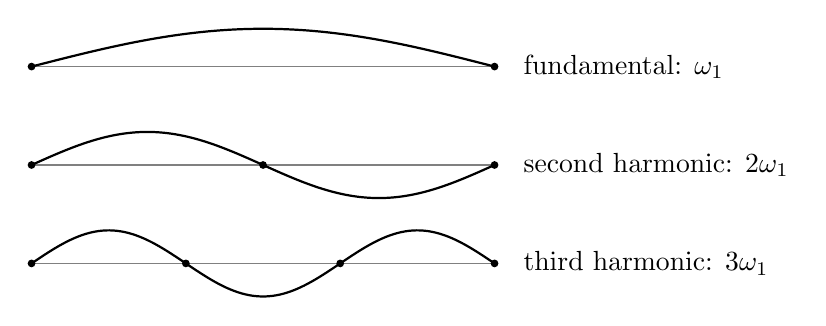
\begin{tikzpicture}[x=0.98cm,y=1cm]
\draw[gray] (0,2.5) -- (6,2.5);
\draw[thick] plot[domain=0:6,samples=120] (\x,{2.5+0.48*sin(30*\x)});
\fill (0,2.5) circle (1.4pt);
\fill (6,2.5) circle (1.4pt);
\node[right] at (6.25,2.5) {fundamental: \(\omega_1\)};

\draw[gray] (0,1.25) -- (6,1.25);
\draw[thick] plot[domain=0:6,samples=120] (\x,{1.25+0.42*sin(60*\x)});
\fill (0,1.25) circle (1.4pt);
\fill (3,1.25) circle (1.4pt);
\fill (6,1.25) circle (1.4pt);
\node[right] at (6.25,1.25) {second harmonic: \(2\omega_1\)};

\draw[gray] (0,0) -- (6,0);
\draw[thick] plot[domain=0:6,samples=120] (\x,{0.42*sin(90*\x)});
\fill (0,0) circle (1.4pt);
\fill (2,0) circle (1.4pt);
\fill (4,0) circle (1.4pt);
\fill (6,0) circle (1.4pt);
\node[right] at (6.25,0) {third harmonic: \(3\omega_1\)};
\end{tikzpicture}%
}
\caption{The string fundamental and its second and third harmonics, with zero, one, and two interior nodes.}
\end{figure}

The fundamental moves as one broad arch and has no interior node. It is one oscillator, and it may contain \(n_1=0,1,2,\ldots\) quanta; each excitation costs \(\hbar\omega_1\). The second harmonic has one interior node and twice the frequency. If the fundamental sounds middle C, this mode sounds the C one octave higher. It has an independent occupation number \(n_2\), and each of its quanta costs \(\hbar\omega_2=2\hbar\omega_1\). The third harmonic has two interior nodes and three times the fundamental frequency. It has its own independent occupation number \(n_3\), which may again be any nonnegative integer.

Mode by mode, in the energy convention used above, the energy is the occupation number times the quantum energy. Collecting those contributions gives
\begin{equation}
E=\sum_{N=1}^{\infty} n_N\hbar\omega_N.
\end{equation}
\editorialnote{This displayed sum is the algebraic collection of the mode energies stated separately at 01:44:02--01:47:46.}

The same harmonic-oscillator mathematics must be repeated for every field mode, with one creation operator and one annihilation operator for each independent oscillator. In this first elementary picture, a quantum field is that entire collection of oscillators and their creation--annihilation algebra.

This language is adapted to particle scattering. Quanta with definite energy and momentum enter an experiment, and quanta with other energies and momenta leave it. The initial particles are removed by annihilation operators; outgoing particles are inserted into the final state by creation operators for the appropriate modes.

\begin{classroomqa}
\lecturetimestamp{01:49:38}
\audiencequestion{Is the same integer being used to label the oscillator mode and to count the number of quanta in it?}
\lecturerresponse{There are two distinct integers. The mode label \(N\) identifies the spatial pattern; in the string example, its number of nodes determines the frequency \(\omega_N\). The occupation number \(n_N\) tells how many quanta have that frequency.}
\end{classroomqa}
